\section{E-Mail}
\begin{frame}{E-Mails: Was soll geschützt werden?}
  E-Mails können
  \begin{itemize}
    \item abgehört
    \item gefälscht
  \end{itemize}
  werden. \pause Deshalb stellen wir vor, wie man
  \begin{itemize}
      \pause
    \item die Vertraulichkeit (das ,,Briefgeheimnis``) umsetzt
    \\ $\Rightarrow$ Verschlüsselung
    \pause
    \item die Echtheit des Gegenübers sicherstellt
    \\ $\Rightarrow$ Digitale Signatur
    \pause
    \item sicherstellt, dass sein E-Mail-Passwort\\ nicht einfach mitgelesen werden kann
  \end{itemize}
\end{frame}

\begin{frame}{Hintergrundinfo Verschlüsselung}
  \framesubtitle{Symmetrische Kryptografie}
  \begin{center}
    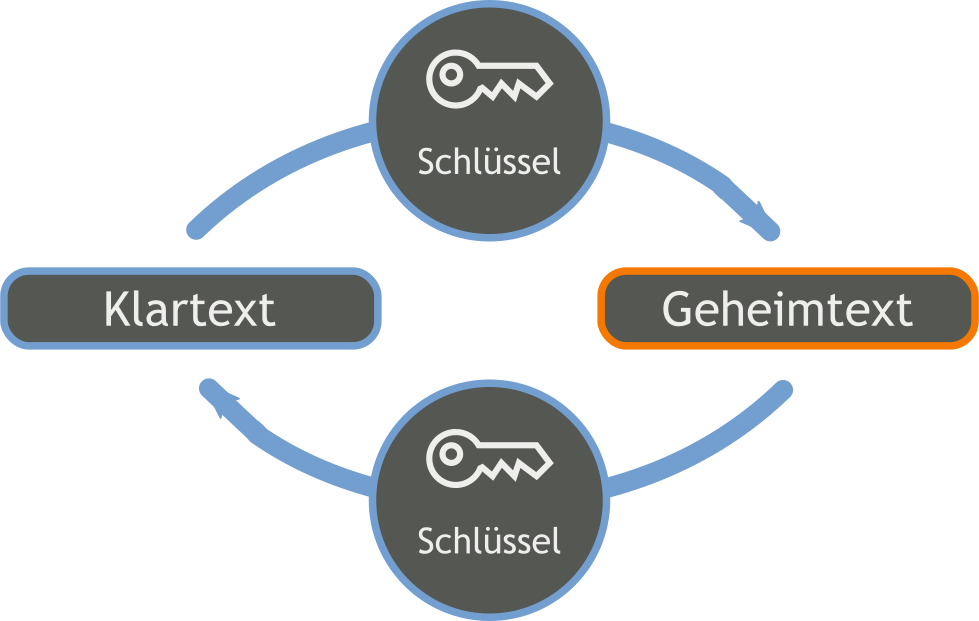
\includegraphics[width=0.5\textwidth]{images/Orange_blue_symmetric_cryptography_de.pdf}
  \end{center}
  \begin{itemize}
    \item Jahrtausende altes Konzept
    \item \emph{Ein} Schlüssel zum Ver- und Entschlüsseln,\\den \emph{alle} Beteiligten kennen
    \item Problem: Schlüsselaustausch
    \begin{itemize}
      \item Wer den Schlüssel kennt, kommt auch an die Daten
      \item Wer den Schlüssel kontrolliert, kontrolliert die Daten
      \begin{itemize}
        \item Ransomware
      \end{itemize}
    \end{itemize}
  \end{itemize}
  \tiny Bildquelle: \href{https://de.wikipedia.org/wiki/Datei:Orange_blue_symmetric_cryptography_de.svg}{,,Symmetrisches Kryptosystem'' von Bananenfalter / CC0}
\end{frame}

\begin{frame}{Hintergrundinfo Verschlüsselung}
  \framesubtitle{Asymmetrische Kryptografie}
  \begin{center}
    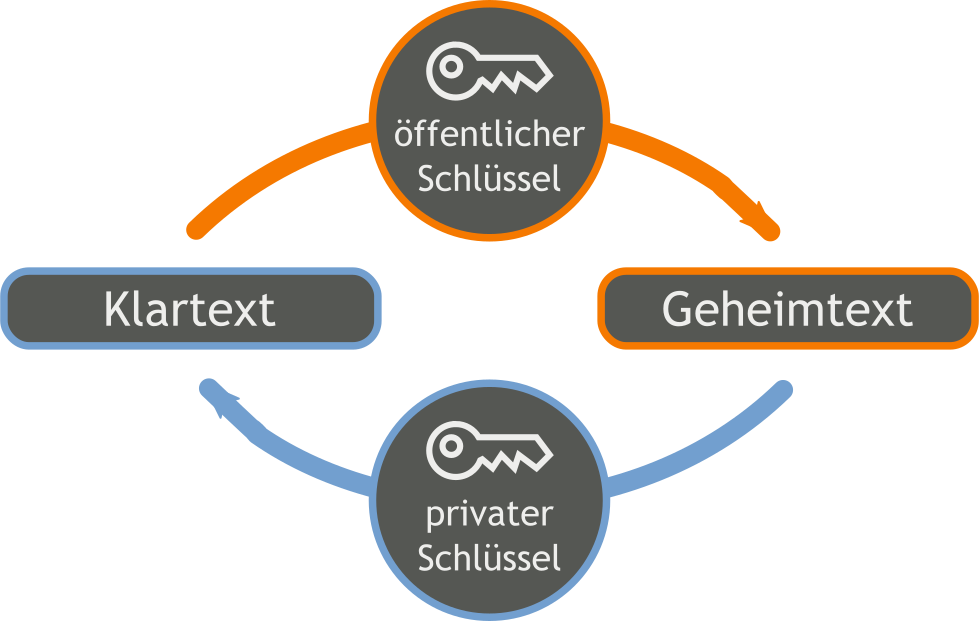
\includegraphics[width=0.5\textwidth]{images/Orange_blue_public_key_cryptography_de.pdf}
  \end{center}
  \begin{itemize}
    \item Prinzip: Schlüssel besteht aus einer \emph{privaten} und einer \emph{öffentlichen} ,,Hälfte``
    \begin{itemize}
      \item Öffentlichen Teil darf/muss man weitergeben
      \item Privaten Teil muss man unbedingt geheim halten
    \end{itemize}
    \item Wird verwendet, um vertraulichen Kanal aufzubauen
    \item Problem weiterhin: Authentizität des öffentlichen Teils
  \end{itemize}
  \tiny Bildquelle: \href{https://commons.wikimedia.org/wiki/File:Orange_blue_public_key_cryptography_de.svg}{,,Asymmetrisches Kryptosystem mit Verschlüsselung und Entschlüsselung'' von Bananenfalter / CC0}
\end{frame}

\begin{frame}{Hintergrundinfo Verschlüsselung}
  \framesubtitle{Asymmetrische Kryptografie -- Anwendungen}
  \begin{itemize}
    \item Verschlüsselung
      \begin{itemize}
        \item Absender \emph{verschlüsselt}\\ mit \emph{öffentlichem} Teil des \emph{Gegenübers}
        \item Nur Gegenüber\\ kann mit \emph{privatem} Gegenstück \emph{entschlüsseln}
      \end{itemize}
    \item Digitale Signatur
      \begin{itemize}
        \item Absender unterschreibt mit \emph{eigenem privaten} Teil
        \item Jeder kann mit \emph{öffentlichem} Gegenstück \emph{überprüfen}
      \end{itemize}
  \end{itemize}
  Es ist mathematisch komplex und benötigt Jahrtausende,\\ um aus einer Signatur oder dem öffentlichen Teil\\ den privaten Teil zu berechnen
\end{frame}
\begin{frame}{E-Mail}{Funktionsweise}
  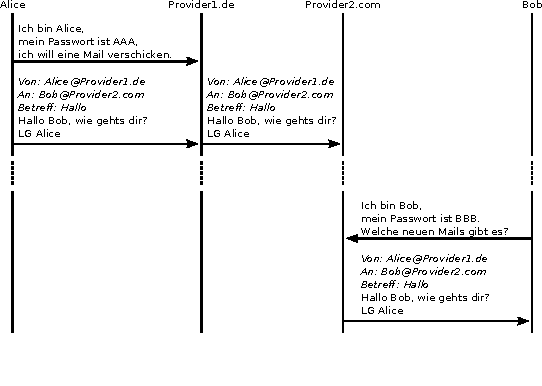
\includegraphics[width=.9\textwidth]{images/maildaten.pdf}
  \scriptsize
  ~\\
  ~\\
\end{frame}

\begin{frame}{E-Mail}{Transportverschlüsselung (SSL/TLS bzw. STARTTLS)}
  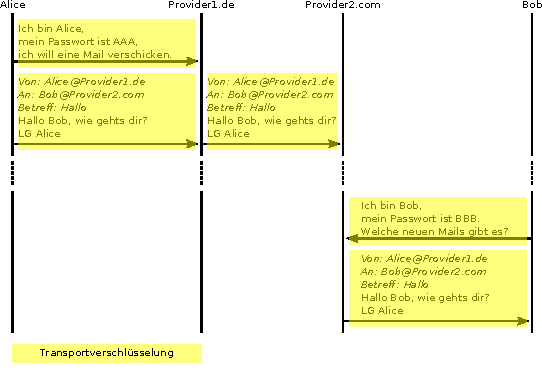
\includegraphics[width=.9\textwidth]{images/maildaten_trans.pdf}
  \begin{itemize}
    \scriptsize
    \item muss von den Mailanbietern unterstützt werden
    \item Konfiguration des Mailprogramms überprüfen!
  \end{itemize}
\end{frame}

\begin{frame}{E-Mail}{Ende-zu-Ende-Verschlüsselung (OpenPGP, S/MIME)}
  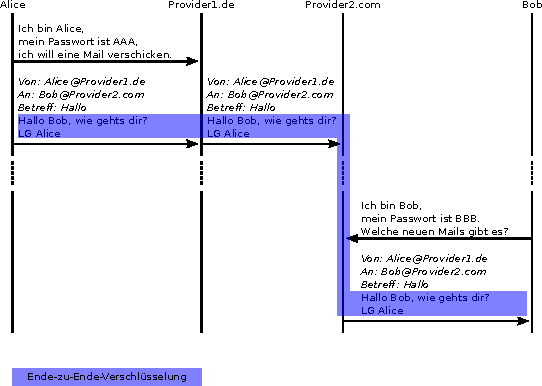
\includegraphics[width=.9\textwidth]{images/maildaten_e2e.pdf}
  \begin{itemize}
    \scriptsize
    \item unabhängig vom Mailanbieter möglich
    \item benötigt Zusatzsoftware und Schlüssel bei beiden Kommunikationspartnern
  \end{itemize}
\end{frame}

\begin{frame}{E-Mail}{Kombination Transport- und Ende-zu-Ende-Verschlüsselung}
  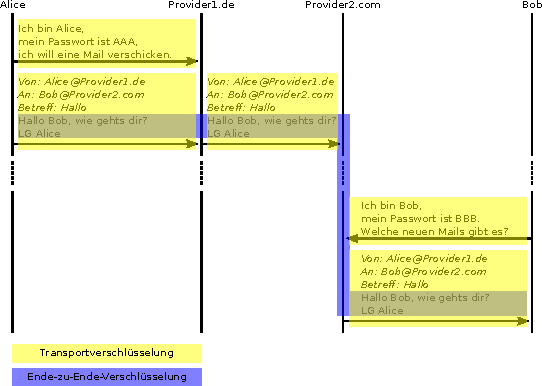
\includegraphics[width=.9\textwidth]{images/maildaten_beides.pdf}
  \scriptsize
  ~\\
  ~\\
\end{frame}

\begin{frame}{Authentizität öffentlicher Schlüssel}
Was, wenn A eine Nachricht an B schicken will,\\ aber den öffentlichen Schlüssel von B nicht kennt?\\
\begin{enumerate}
  \item Im ``Telefonbuch'' nach dem Schlüssel suchen
  \item Echtheit mit Hilfe eines \emph{vertrauenswürdigen Dritten} C überprüfen
\end{enumerate}
\begin{center}
  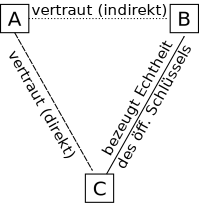
\includegraphics[width=0.5\textheight]{images/vertrauen.pdf}
  %TODO: überarbeiten
\end{center}
\end{frame}

\begin{frame}{Wie stellt man Vertrauen in öffentliche Schlüssel her?}
  \begin{itemize}
    \item S/MIME -- Hierarchischer Vertrauensansatz
    \begin{itemize}
      \item hier nicht behandelt
    \end{itemize}
    \item OpenPGP -- Dezentraler Vertrauensansatz
    \begin{itemize}
      \item jeder kann festlegen, wem er vertraut
      \begin{itemize}
        \item er kann die Echtheit eines Schlüssels\\ z.B. bei einem persönlichen Treffen überprüfen
      \end{itemize}
      \item jeder \emph{kann} sein Vertrauensnetz veröffentlichen (Web-of-Trust)
      \begin{itemize}
        \item Vorteil: Man kann ``Freunden von Freunden'' vertrauen
        \item Nachteil: Beziehungen zwischen Menschen öffentlich\\ Aber: Facebook sagt da viel mehr aus
      \end{itemize}
      %\item wird hier behandelt
    \end{itemize}
  \end{itemize}
\end{frame}

\begin{frame}{Welche Software benötigt man?}
  \begin{block}{OpenPGP Backend}
    Macht die eigentliche Ver-/Entschlüsselung \& Signatur

    \vspace{1ex}
    \begin{tabular}{ccc}
      Linux:            & Windows: & Android:     \\
      \textit{on-board} & GPG4Win  & OpenKeychain \\
    \end{tabular}
  \end{block}
  \begin{block}{Plug-In fürs Mailprogram}
    Grafische Oberfläche, leichtere Schlüsselverwaltung, etc.

    \vspace{1ex}
    \begin{tabular}{ccc}
      Thunderbird: & Outlook: & K9-Mail: \\
      Enigmail     & GPG4Win  & --       \\
    \end{tabular}
  \end{block}
\end{frame}

\endinput
